\chapter{System Maintenance}

\section{Environment}

\subsection{Software}
In the process of creating my code, I used the following programs: 
\begin{itemize}
	\item Python 3.4
	\item PyQt4
	\item Python IDLE
	\item SQLite3
	\item SQLite Inspector
\end{itemize}
\subsection{Usage Explanation}
I used Python 3.4 because it has syntax that is similar to pseudocode, meaning it is easier to learn than some other languages. 

PyQt4 is the GUI extension to Python 3.4, and offers a huge library of UI elements that are all fully documented online. For this reason I used PyQt4. 

Python Integrated Development Environement, or IDLE, allowed me to write Python 3.4 code, while colour coding the different types of syntax, making the code easier to read. This was especially useful to me when my program started to become very large, the colour coding made it easier to pick our elements of the code. Also, IDLE was a platform for me to run my program on, and it returned any program errors/crashes, and allowed me to view which line the program crashed on, or which line threw an error. 

SQLite3 is a language for interacting with SQLite databases, and can be imported directly into Python 3.4 scripts, (See figure \ref{fig:Import SQLite3 into Python 3.4} and  figure \ref{fig:Example SQLite3 code in Python 3.4}) and so was essential to creating and interacting with a database.

\begin{figure}[H]
    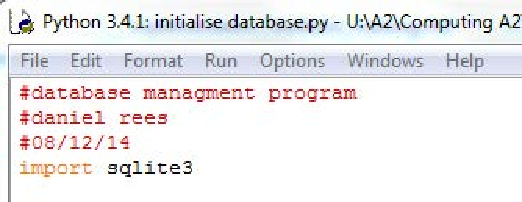
\includegraphics[width=\textwidth]{./Maintenance/Import_SQLite3.pdf}
    \caption{Importing the SQLite3 module directly into a Python 3.4 Script} \label{fig:Import SQLite3 into Python 3.4}
\end{figure}
\begin{figure}[H]
    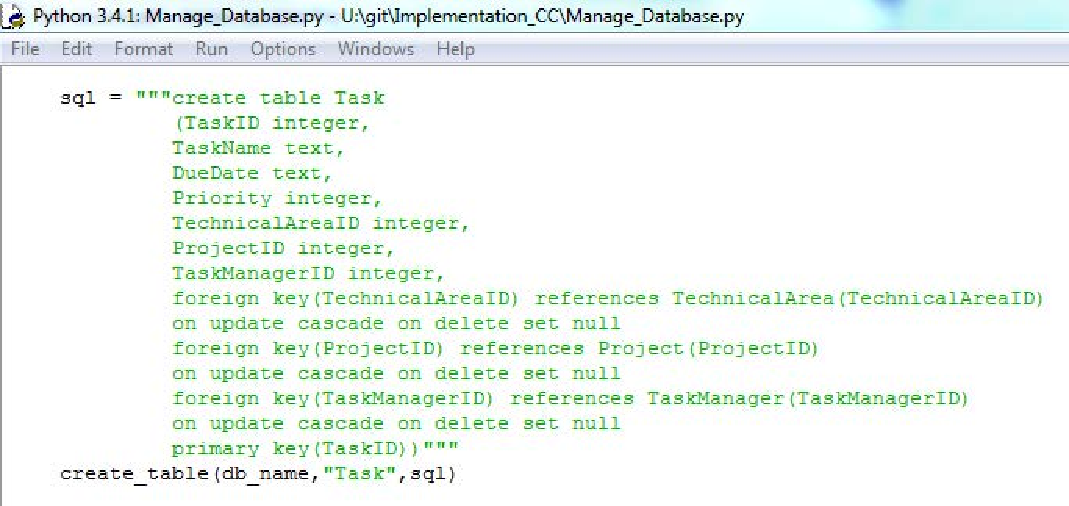
\includegraphics[width=\textwidth]{./Maintenance/Example_SQLite3_Code.pdf}
    \caption{Using SQLite3 code in the Python 3.4 IDLE} \label{fig:Example SQLite3 code in Python 3.4}
\end{figure}

SQLite Inspector is a database viewing program whcih allows you to view the entity descriptions of a database (see figure \ref{fig:SQLite Inspector Entity Descriptions}), and view the data in each table of the database (see figure \ref{fig:SQLite Inspector Table Data}),execute queries on a given database (see figure \ref{ig:SQLite Inspector Query}). 

\begin{figure}[H]
    \includegraphics[width=\textwidth]{./Maintenance/SQLite_Inspector_Entitydesc_Example.pdf}
    \caption{Viewing the Entity Descriptions of a database} \label{fig:SQLite Inspector Entity Descriptions}
\end{figure}
\begin{figure}[H]
    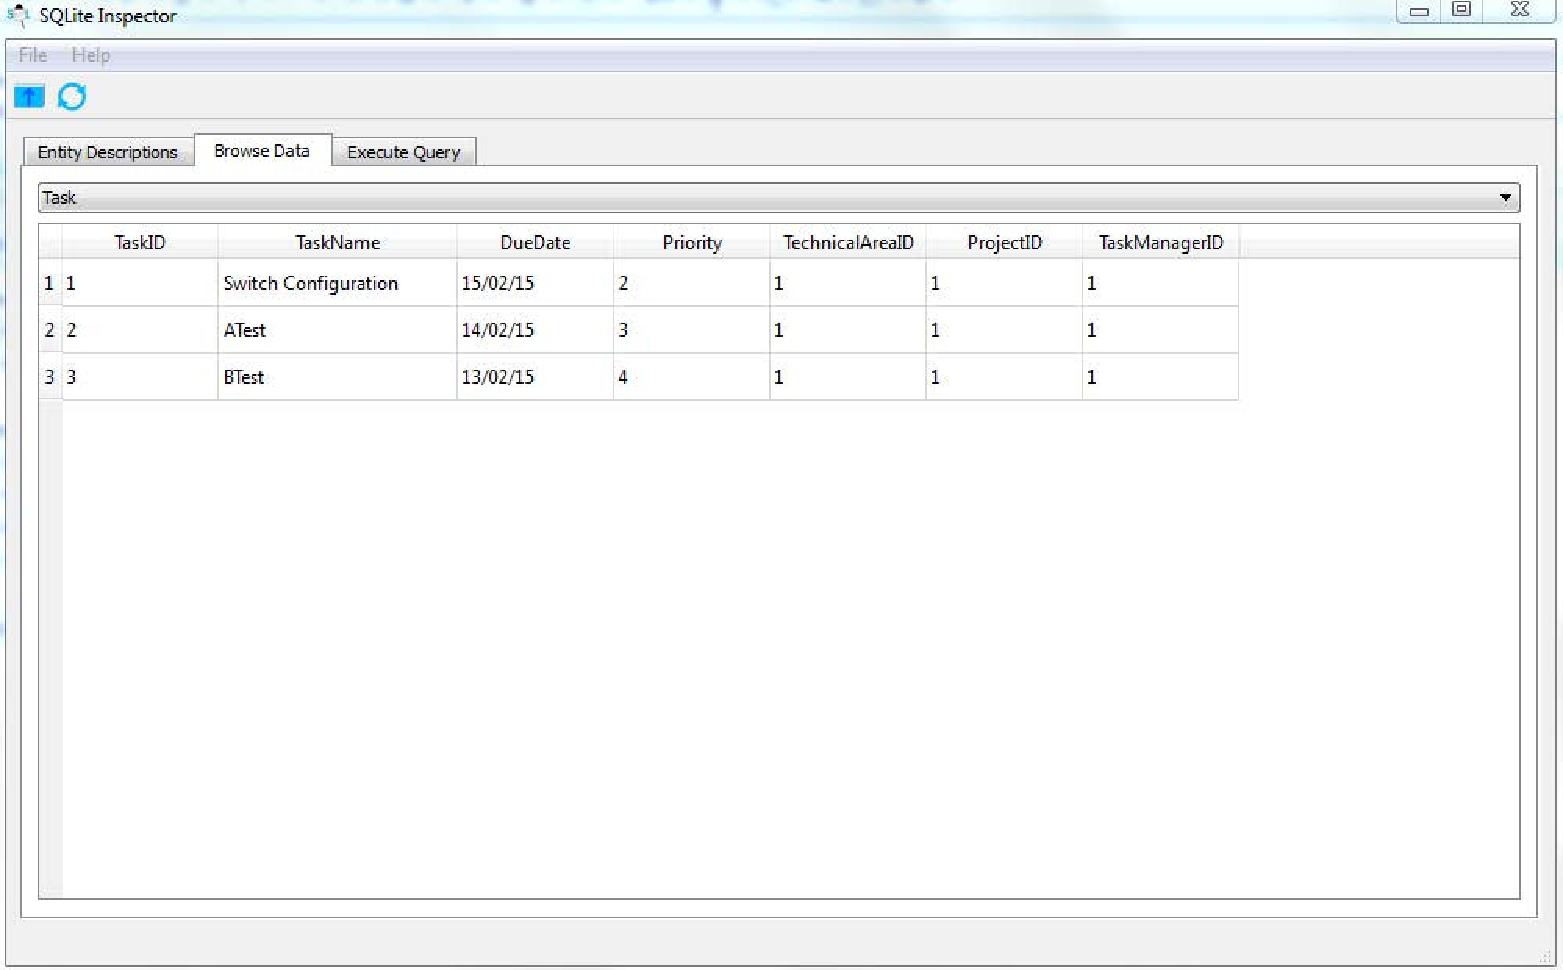
\includegraphics[width=\textwidth]{./Maintenance/SQLite_Inspector_Viewtable_Example.pdf}
    \caption{Viewing the data in the table of a database} \label{fig:SQLite Inspector Table Data}
\end{figure}
\begin{figure}[H]
    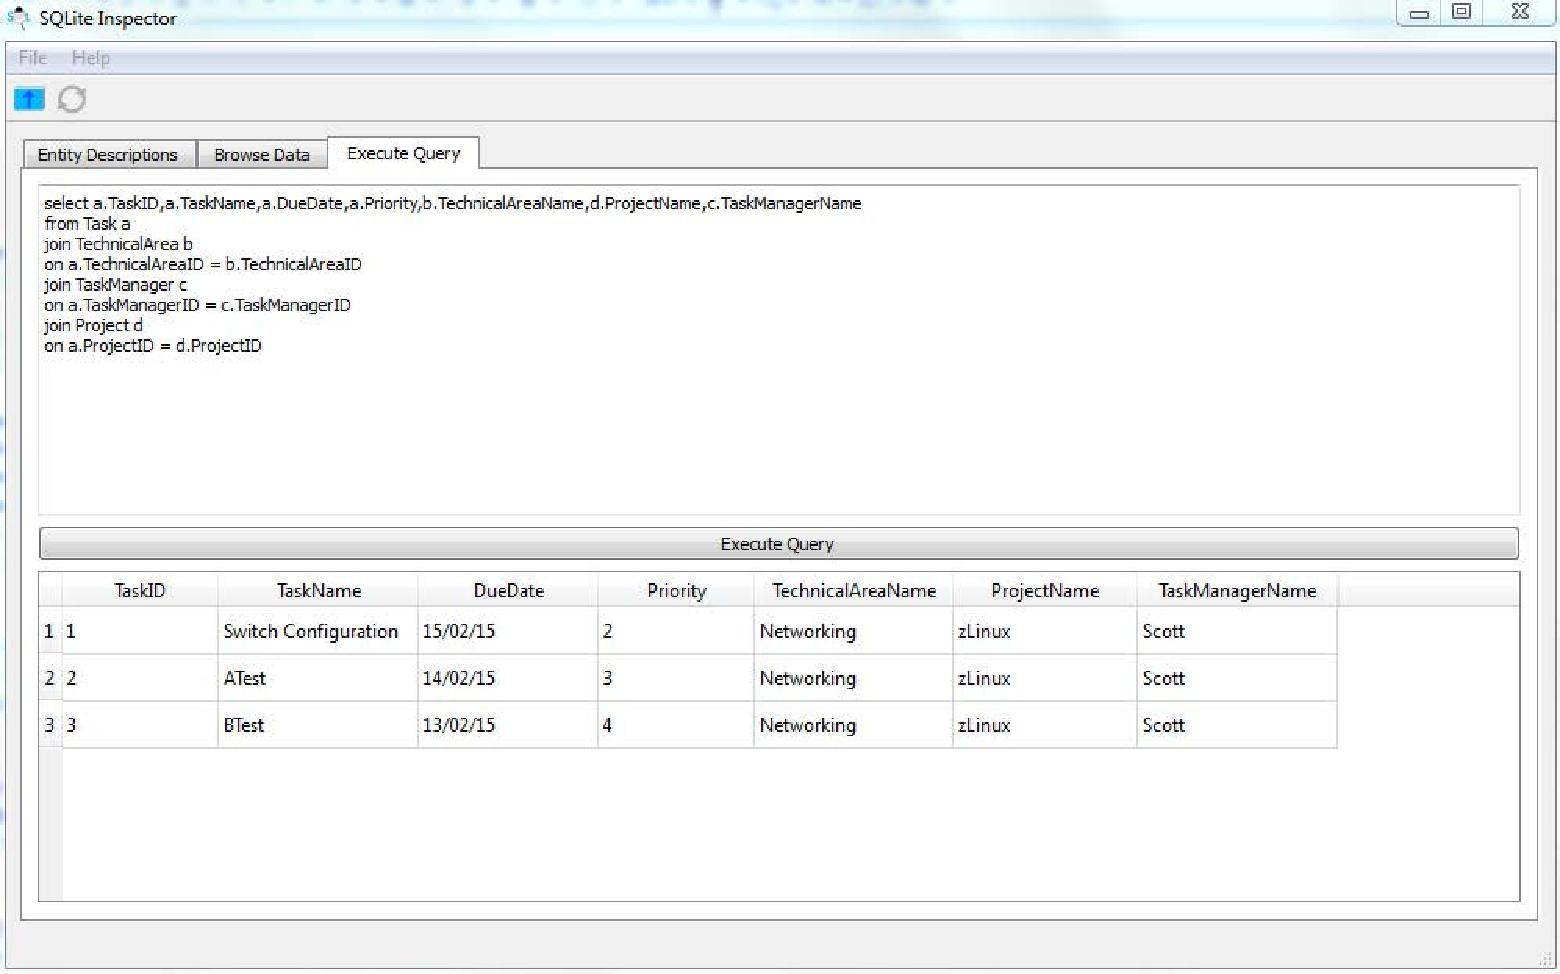
\includegraphics[width=\textwidth]{./Maintenance/SQLite_Inspector_Query_Example.pdf}
    \caption{Executing a Query on a database} \label{fig:SQLite Inspector Query}
\end{figure}

\subsection{Features Used}

\section{System Overview}

%use as many subsections as necessary for the system components
\subsection{System Component}

\section{Code Structure}

%use as many subsections as necessary for the code sections
\subsection{Particular Code Section}
%the code below can be uncommented and used to get a code section from a particular file
\begin{comment}
\begin{figure}[H]
    \pythonfile[firstline=5,lastline=10]{./tex/function_programs/print_function.py}
    \caption{The print() function} \label{fig:print_function}
\end{figure}
\end{comment}

\section{Variable Listing}

\section{System Evidence}

\subsection{User Interface}

\subsection{ER Diagram}

\subsection{Database Table Views}

\subsection{Database SQL}

\subsection{SQL Queries}

\section{Testing}

\subsection{Summary of Results}

\subsection{Known Issues}

\section{Code Explanations}

\subsection{Difficult Sections}

\subsection{Self-created Algorithms}

\section{Settings}

\section{Acknowledgements}

\section{Code Listing}
\begin{landscape}
%include as many subsections as you have modules
\subsection{Module 1}
%the code below can be uncommented and used to get a code section from a particular file
\begin{comment}
\pythonfile[firstline=5]{./tex/function_programs/print_function.py}
\end{comment}
\end{landscape}
